\documentclass{standalone}
\usepackage{tikz}
\usetikzlibrary{patterns, positioning}
\usetikzlibrary{shapes.misc}
\usepackage[outline]{contour}
\contourlength{1.5pt} 
\usepackage[sfdefault]{ClearSans} %% option 'sfdefault' activates Clear Sans as the default text font
\usepackage[T1]{fontenc}

\begin{document}
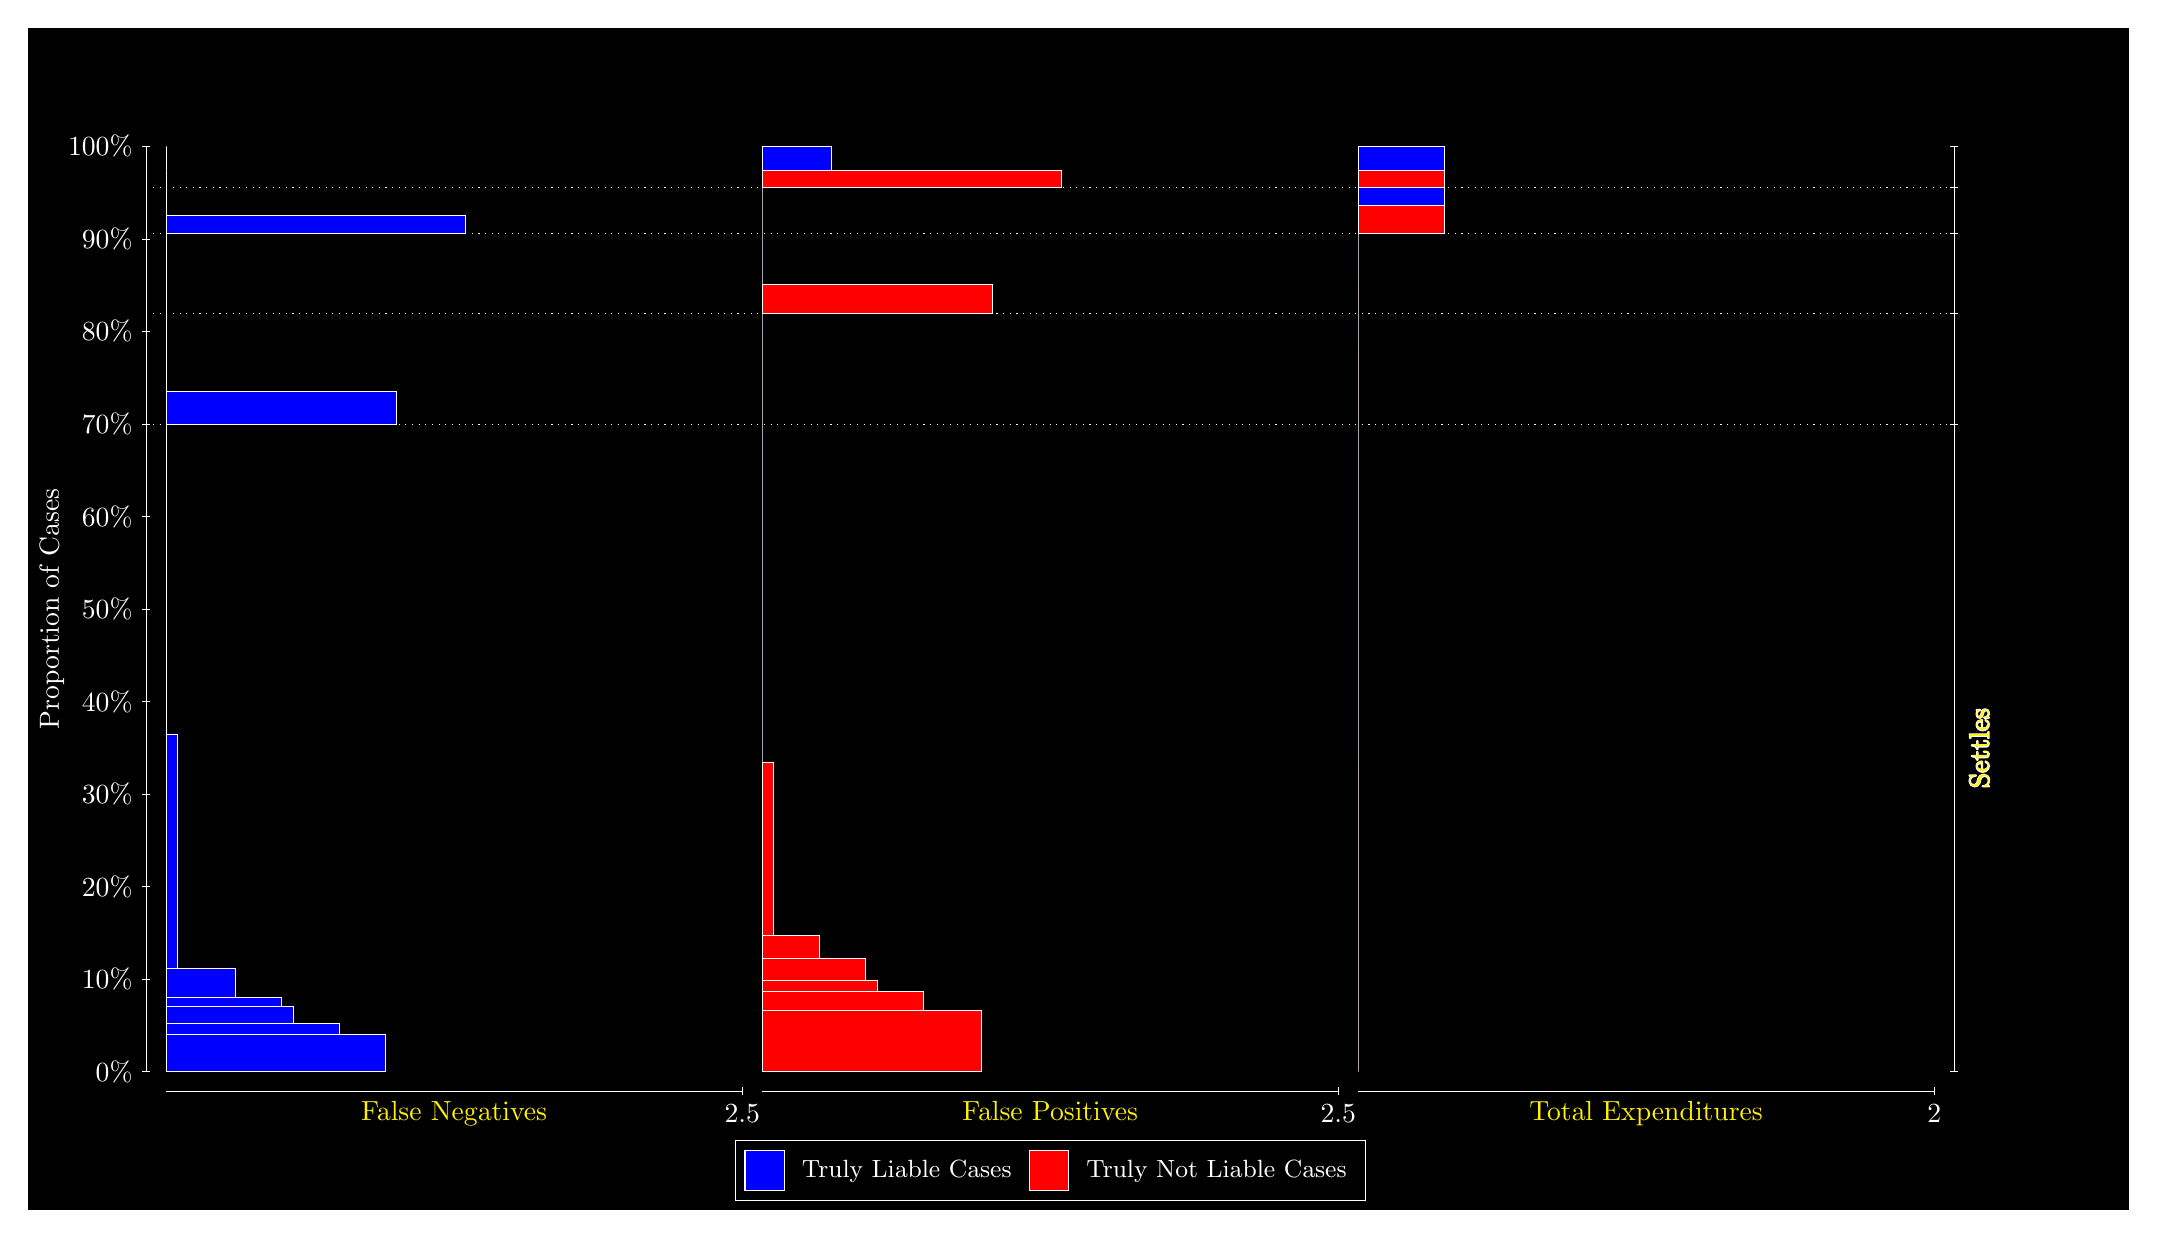
\begin{tikzpicture}
\draw[fill=black] (0,0) rectangle (26.667,15);
\draw[white, very thin] (1.5,1.75) -- (1.5,13.5);
\node[rotate=90, text=white, anchor=center] at (0.3, 7.625) {Proportion of Cases};
\draw[white, very thin] (1.45,1.75) -- (1.55,1.75);
\node[text=white, anchor=east] at (1.45, 1.75) {0\%};
\draw[white, very thin] (1.45,2.925) -- (1.55,2.925);
\node[text=white, anchor=east] at (1.45, 2.925) {10\%};
\draw[white, very thin] (1.45,4.1) -- (1.55,4.1);
\node[text=white, anchor=east] at (1.45, 4.1) {20\%};
\draw[white, very thin] (1.45,5.275) -- (1.55,5.275);
\node[text=white, anchor=east] at (1.45, 5.275) {30\%};
\draw[white, very thin] (1.45,6.45) -- (1.55,6.45);
\node[text=white, anchor=east] at (1.45, 6.45) {40\%};
\draw[white, very thin] (1.45,7.625) -- (1.55,7.625);
\node[text=white, anchor=east] at (1.45, 7.625) {50\%};
\draw[white, very thin] (1.45,8.8) -- (1.55,8.8);
\node[text=white, anchor=east] at (1.45, 8.8) {60\%};
\draw[white, very thin] (1.45,9.975) -- (1.55,9.975);
\node[text=white, anchor=east] at (1.45, 9.975) {70\%};
\draw[white, very thin] (1.45,11.15) -- (1.55,11.15);
\node[text=white, anchor=east] at (1.45, 11.15) {80\%};
\draw[white, very thin] (1.45,12.325) -- (1.55,12.325);
\node[text=white, anchor=east] at (1.45, 12.325) {90\%};
\draw[white, very thin] (1.45,13.5) -- (1.55,13.5);
\node[text=white, anchor=east] at (1.45, 13.5) {100\%};

\draw[white, very thin] (24.457,1.75) -- (24.457,13.5);
\draw[white, very thin] (24.407,1.75) -- (24.507,1.75);
\node[anchor=west] at (24.407, 1.75) {};
\draw[white, very thin] (24.407,9.9638) -- (24.507,9.9638);
\node[anchor=west] at (24.407, 9.9638) {};
\draw[white, very thin] (24.407,11.382) -- (24.507,11.382);
\node[anchor=west] at (24.407, 11.382) {};
\draw[white, very thin] (24.407,12.393) -- (24.507,12.393);
\node[anchor=west] at (24.407, 12.393) {};
\draw[white, very thin] (24.407,12.981) -- (24.507,12.981);
\node[anchor=west] at (24.407, 12.981) {};
\draw[white, very thin] (24.407,13.5) -- (24.507,13.5);
\node[anchor=west] at (24.407, 13.5) {};

\draw[white, very thin, fill=blue] (1.75,1.75) rectangle (4.5312,2.2241);
\draw[white, very thin, fill=blue] (1.75,2.2241) rectangle (3.9457,2.3577);
\draw[white, very thin, fill=blue] (1.75,2.3577) rectangle (3.3602,2.5838);
\draw[white, very thin, fill=blue] (1.75,2.5838) rectangle (3.2138,2.6953);
\draw[white, very thin, fill=blue] (1.75,2.6953) rectangle (2.6283,3.0554);
\draw[white, very thin, fill=blue] (1.75,3.0554) rectangle (1.8964,6.0334);
\draw[white, very thin, fill=red] (1.75,6.0334) rectangle (1.75,9.9638);
\draw[white, very thin, fill=blue] (1.75,9.9638) rectangle (4.6775,10.386);
\draw[white, very thin, fill=red] (1.75,10.386) rectangle (1.75,11.382);
\draw[white, very thin, fill=red] (1.75,11.382) rectangle (1.75,11.753);
\draw[white, very thin, fill=blue] (1.75,11.753) rectangle (1.75,12.393);
\draw[white, very thin, fill=blue] (1.75,12.393) rectangle (5.5558,12.619);
\draw[white, very thin, fill=red] (1.75,12.619) rectangle (1.75,12.981);
\draw[white, very thin, fill=red] (1.75,12.981) rectangle (1.75,13.196);
\draw[white, very thin, fill=blue] (1.75,13.196) rectangle (1.75,13.5);
\draw[white, very thin, fill=red] (9.3189,1.75) rectangle (12.1,2.5289);
\draw[white, very thin, fill=red] (9.3189,2.5289) rectangle (11.368,2.7743);
\draw[white, very thin, fill=red] (9.3189,2.7743) rectangle (10.783,2.911);
\draw[white, very thin, fill=red] (9.3189,2.911) rectangle (10.636,3.1873);
\draw[white, very thin, fill=red] (9.3189,3.1873) rectangle (10.051,3.4778);
\draw[white, very thin, fill=red] (9.3189,3.4778) rectangle (9.4652,5.6804);
\draw[white, very thin, fill=blue] (9.3189,5.6804) rectangle (9.3189,9.9638);
\draw[white, very thin, fill=red] (9.3189,9.9638) rectangle (9.3189,10.96);
\draw[white, very thin, fill=blue] (9.3189,10.96) rectangle (9.3189,11.382);
\draw[white, very thin, fill=red] (9.3189,11.382) rectangle (12.246,11.753);
\draw[white, very thin, fill=blue] (9.3189,11.753) rectangle (9.3189,12.393);
\draw[white, very thin, fill=red] (9.3189,12.393) rectangle (9.3189,12.755);
\draw[white, very thin, fill=blue] (9.3189,12.755) rectangle (9.3189,12.981);
\draw[white, very thin, fill=red] (9.3189,12.981) rectangle (13.125,13.196);
\draw[white, very thin, fill=blue] (9.3189,13.196) rectangle (10.197,13.5);
\draw[white, very thin, fill=red] (16.888,1.75) rectangle (16.888,5.6804);
\draw[white, very thin, fill=blue] (16.888,5.6804) rectangle (16.888,9.9638);
\draw[white, very thin, fill=red] (16.888,9.9638) rectangle (16.888,10.96);
\draw[white, very thin, fill=blue] (16.888,10.96) rectangle (16.888,11.382);
\draw[white, very thin, fill=red] (16.888,11.382) rectangle (16.888,11.753);
\draw[white, very thin, fill=blue] (16.888,11.753) rectangle (16.888,12.393);
\draw[white, very thin, fill=red] (16.888,12.393) rectangle (17.986,12.755);
\draw[white, very thin, fill=blue] (16.888,12.755) rectangle (17.986,12.981);
\draw[white, very thin, fill=red] (16.888,12.981) rectangle (17.986,13.196);
\draw[white, very thin, fill=blue] (16.888,13.196) rectangle (17.986,13.5);
\draw[white, dotted] (1.5,9.9638) -- (24.457,9.9638);
\draw[white, dotted] (1.5,11.382) -- (24.457,11.382);
\draw[white, dotted] (1.5,12.393) -- (24.457,12.393);
\draw[white, dotted] (1.5,12.981) -- (24.457,12.981);
\draw[white, very thin] (1.75,1.5) -- (9.0689,1.5);
\node[text=yellow, anchor=north] at (5.4094, 1.5) {False Negatives};
\draw[white, very thin] (9.0689,1.45) -- (9.0689,1.55);
\node[text=white, anchor=north] at (9.0689, 1.45) {2.5};

\draw[white, very thin] (9.3189,1.5) -- (16.638,1.5);
\node[text=yellow, anchor=north] at (12.978, 1.5) {False Positives};
\draw[white, very thin] (16.638,1.45) -- (16.638,1.55);
\node[text=white, anchor=north] at (16.638, 1.45) {2.5};

\draw[white, very thin] (16.888,1.5) -- (24.207,1.5);
\node[text=yellow, anchor=north] at (20.547, 1.5) {Total Expenditures};
\draw[white, very thin] (24.207,1.45) -- (24.207,1.55);
\node[text=white, anchor=north] at (24.207, 1.45) {2};

\node[text=yellow, centered, rotate=90] at (24.777, 5.8569) {\contour{white}{Settles}};





\draw (12.978300999999998,1.5) node[draw=none] (baseCoordinate) {};
\begin{scope}[align=center]
        \matrix[scale=0.5, draw=white, below=0.5cm of baseCoordinate, nodes={draw}, column sep=0.1cm]{
            \node[rectangle, draw, minimum width=0.5cm, minimum height=0.5cm, fill=blue] {}; &
            \node[draw=none, font=\small, text=white] (B) {Truly Liable Cases}; &
            \node[rectangle, draw, minimum width=0.5cm, minimum height=0.5cm, fill=red] {}; &
            \node[draw=none, font=\small, text=white] (B) {Truly Not Liable Cases}; \\
            };
\end{scope}

\end{tikzpicture}
\end{document}